\documentclass{article}
\usepackage[utf8]{inputenc}

\title{Materials and Designs for Drones and Ornithopters}
\author{Aakash \\ Email: \href{mailto:me16b001@iittp.ac.in}{me16b001@iittp.ac.in}}
\date{March 2019}
 \usepackage{hyperref}
\usepackage{natbib}
\usepackage{graphicx}

\begin{document}

\maketitle

\begin{abstract}
In this term-paper we present a review of the advancements in materials and designs for drones as well as ornithopters. We also provide a detailed description of the drones, their categorization, and the types of possible materials that can be used for the light-weight application for the drones, increasing their efficiency and time of flight.
\end{abstract}

\section{Introduction}
In recent years, the use of Unmanned Aerial Vehicles(UAV) is playing important roles in different applications. Commonly known as a drone, a UAV is an aircraft that can perform flight missions autonomously without the requirement of a human pilot onboard, or can be tele-operated by a pilot from a ground station. It is used in many aspects of military and civil broadly, such as aerial photogrammetry, agriculture, warzone, surveillance, traffic and climate monitoring and so on. These stealth crafts are becoming increasingly popular, not just for war and military purposes, but also for everything from wildlife and atmospheric research to disaster relief and sports photography. Drones are becoming extremely usefull for scientists in order to carry out surveying for archaeological sites, monitor signs of illegal hunting and crop damage, and even zipping inside hurricanes to study the wild storms. 
Unmanned aerial vehicle (UAV) research and development has been growing rapidly ever since over the past decade. One of the important aspect in the design of the drones is the selection of the right material, the material has to be strong enough to provide it rigidity, it should be aerodynamic and light weight at the same time for longer and efficient time of flight.  

A flapping-wing UAV, commonly known as an ornithopter in the literature, usually is about a hand size although the size may vary a lot depending on the type of application it has been developed for. It generates required lifting and forward force by mainly by flapping its wings. The aerodynamic modelling and simulation of the ornithopter is much more involved \citep{peterson}. This requires knowledge from different domains such as fluid mechanics, material science, electrical engineering and of course computer science in order to devlop the required control and algorithm.

In the beginning sections we provide an overview of the advancements in design and material selection for the drones or UAVs. Later section follows the overview of the much recent advancement i.e. the ornithopters, although there have been some successful models still this area is under research and development. In the final section we provide the conclusions.

\section{Designing of Drones}
There are different types of drone designs are available in the market but the two most common types of drones are shown in Figure ~\ref{fig:drone} and ~\ref{fig:drone2}, the one in Figure ~\ref{fig:drone} shows the fixed wing drone with rotors for providing the required lift and control (roll, pitch, yaw) while the one in the Figure ~\ref{fig:drone2} shows a fixed wing type drone. The fixed wing drone, consists of a fixed and rigid wing that has an airfoil shape which generates the  lift in presence of some airspeed which is generated by a propeller. The control mainly consists of a rudder, ailerons, elevators. 

UAV design and advancement is a global activity, and an very active area of research.  As we adopt more and more advanced technologies like - computer vision, Machine Learning and Artificial Intelligence into these machines they are getting more and more advanced and acurate in their tasks. In this paper however we will only be covering the mechanical design aspects and the advance-ments in materials. It is important to make the body and the supporting structures as light as possible, therefore the lightest, and most cost effective materials available are to be considered. One of the most popular types of materials are the composites and fiber reinforced materials. 

In the following subsection we discuss the various available materials for drones while in the latter we throw some light in the desining of drones.

\begin{figure}
    \centering
    \begin{minipage}{0.45\textwidth}
        \centering
        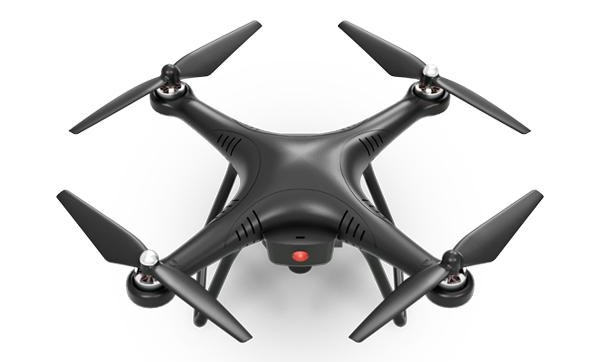
\includegraphics[width=0.9\textwidth]{drone.jpg} % first figure itself
        \caption{Common drone}
        \label{fig:drone}
    \end{minipage}\hfill
    \begin{minipage}{0.45\textwidth}
        \centering
        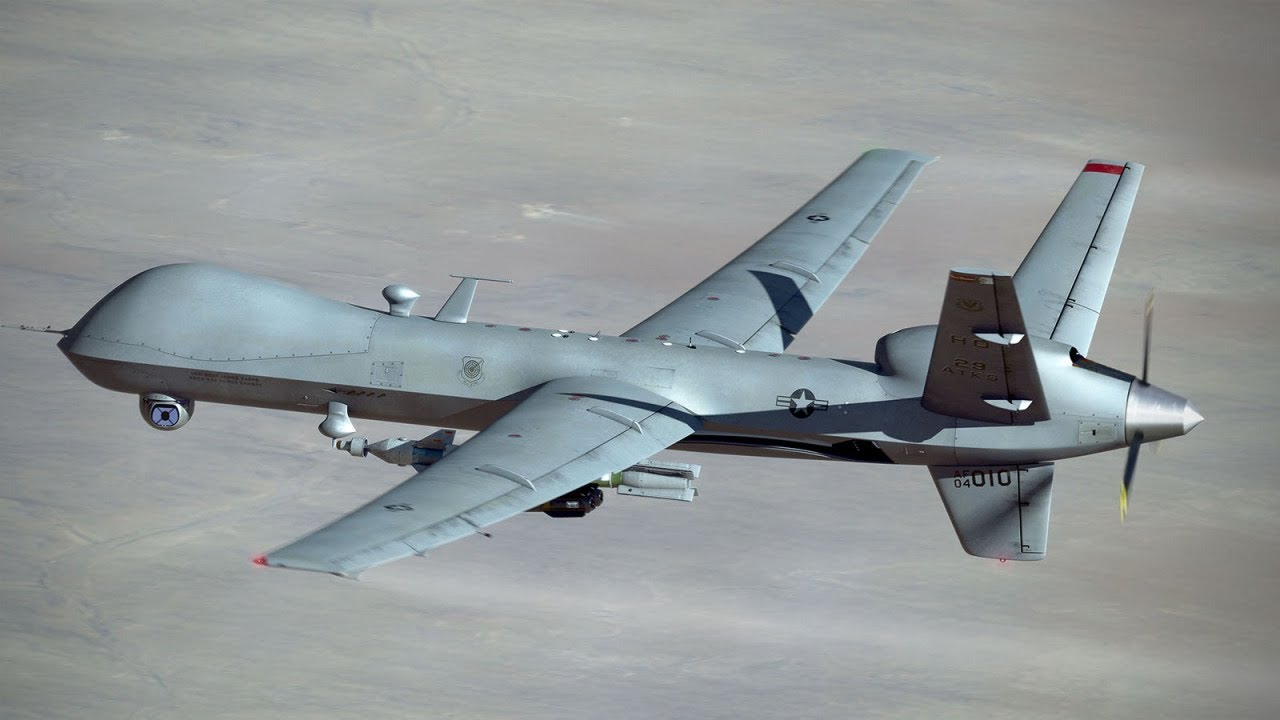
\includegraphics[width=0.9\textwidth]{drone2.jpg} % second figure itself
        \caption{Military drone}
        \label{fig:drone2}
    \end{minipage}
\end{figure}

\subsection{Composite materials}

A composite material in general is made by combination of two or more materials, many a times both having quite different  different properties. The two materials work together to give the composite unique properties. The materials are binded together by suitable binders. 

In the present scenario there is a very high requirement for the modern drones  to use composite materials (high strength-low weight), specially polymer matrix composites reinforced with continuous fibers are one of the most  appropriate choices \citep{kassapoglou}. The fibres help the material bind better and result in a stronger material do to reinforcement, the fibres also help in taking the tensile loads wherever applicable. These materials can be  characterized by Young's module twice as high when compared with aluminum alloys while retaining two times lower weight. The difficulties in use of composites materials are related to the anisotropic or orthotropic structure. Performing numerical analysis and simulations for these materials requires sound knowledge of material constants and mechanical properties in principal axes along with the expertise in solid mechanics. The structural reliability can only be guaranted after sound calculations of the fully defined composite material \citep{chung}.

Commonly available composite materials generally consist of two or more phases having remarkably vivid properties, both physical and chemical. Combined together they form a material having characteristics different from individual components. Each phase remain separate within the finished structure. Based on the function played the different components, they can be divided into either filler (reinforcement) or  matrix. Mostly used matrices materials are polymers, metals, ceramics and carbon while fillers materials are glass, carbon, aramid and boron. Reinforcement occur in different forms such as continues fibers, short fibers and particles. Figure ~\ref{fig:binding}  shows the possible reinforcement types  \citep{Chandramohan2018}.

\begin{figure}[h!]
\centering
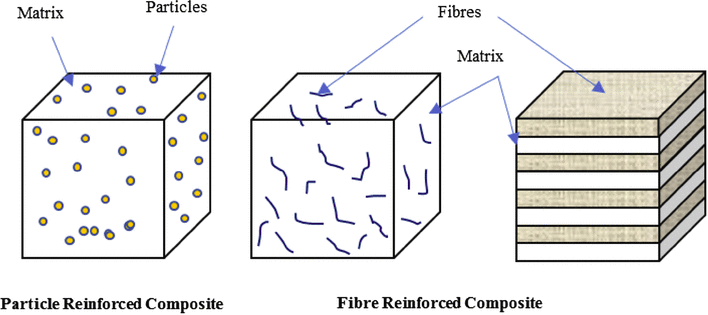
\includegraphics[scale=0.5]{binding.png}
\caption{ Types of reinforcements (Chandramohan et al)}
\label{fig:binding}
\end{figure}

One of the most common composites are the polymer matrix composites. They provide good properties such as high stiffness, low density, high strength, corrosion resistance and vibration damping ability, moreover they have low  fabrication costs. The most common materials used are vinyl ester, epoxy, phenol, formaldehyde, polyamide, polyimide and polypropylene  resins. The most frequent occurring types of fabrics used as reinforcement for polymer composites are plain weave, twill wave and unidirectional fabric. \citep{krolikowski}.

Another type of composite is the polymer matrix composites, it commonly occurs in form of symmetrical and asymmetrical laminates. Laminates are formed by bonding of fibrous composites layers together, it provides the required engineering properties to the material. Different material properties can be achieved by changing the orientation of the laminate layers.

\begin{figure}[h!]
\centering
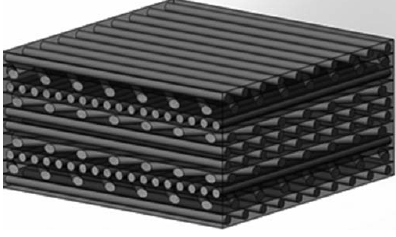
\includegraphics[scale=0.5]{dfm2}
\caption{ Composite laminate with different layer orientations}
\end{figure}
\subsection{Design of static wing for drones}

Designing of the wings is undoublty the most imortant yet critical task while designing a fixed wing drone, the properties such as airfoil shape, thickness, chords dimensions, span, surface area and geometry of the wings vary across its length making its analysis and simulation complicated (The workflow is shown in the  Figure ~\ref{fig:drone2}.
\begin{figure}[h!]
\centering
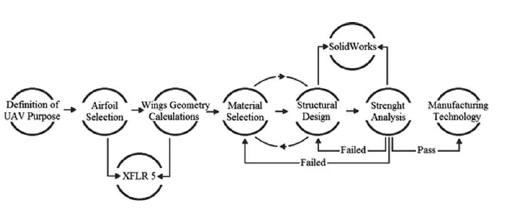
\includegraphics[scale=0.5]{workflow.png}
\caption{Process flow for designing of a fixed type wing (Andrzej et al)}
\end{figure}

It is important to have knowledge about different types of loads acting on designed element while designing the same and selecting materials for the same. In case of design process for UAV wing structures most important loads that are acting on the structure are bending loads and torsion loads derived from acting lift force. Due to high requirements of the modern UAV’s (high strength-low weight) composite materials especially polymer matrix composites reinforced with continues fibers are most appropriate choice. The wing geometry design can be carried out in XFLR 5 software. We are required to carry out detailed numerical simulation of the wing for load and temperature changes it may have to undergo during its time of flight.

\begin{figure}[h!]
\centering
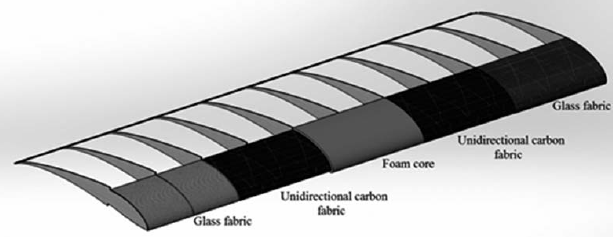
\includegraphics[scale=0.5]{dfm3}
\caption{ Structural design of UAV wing}
\end{figure}

\section{Designing of Ornithopter's flapping Mechanisms}

Ornithopter is one of the most demanded drone types in todays world, one of the reasons it having the ability to camouflage in the environment. Many of the wing designs for ornithopters are inspired by the real birds, because natures promises very efficient designs. Sutthiphong et al
\citep{Sutthiphong} provides a very elaborative process of wing design inspired by albatross (a long distance migratory birds). Moreover the ornithopters are required to be packed by loadful of sensors and imaging cameras to carry out the tasks both for military and civilian surveillance. One of the common design for ornithopters i.e. flapping wing provides us with a sophisticated example of utilizing unsteady aerodynamics for mechanizing the wing design for low reynolds numbers. The design process typically divided into design aspects related to different disciplines, it includes design for mechanisms (Design of machinery), design for aerodynamics and fluid flow modelling and desgin considering the material aspect.
Figure  ~\ref{fig:p2} shows the crude mechanical design for the flapping wing mechanism, while the figure  ~\ref{fig:p1} shows the design prototype.

\begin{figure}
    \centering
    \begin{minipage}{0.5\textwidth}
        \centering
        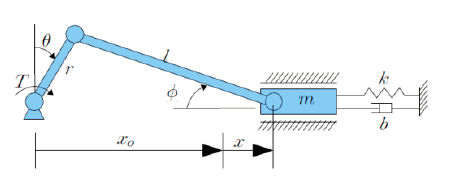
\includegraphics[width=0.9\textwidth]{p2.png} % first figure itself
    \end{minipage}\hfill
    \begin{minipage}{0.5\textwidth}
        \centering
        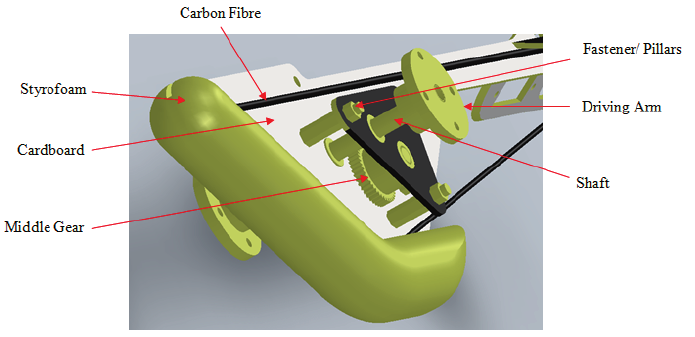
\includegraphics[width=0.9\textwidth]{p3.png} % second figure itself
    \end{minipage}
\caption{ Flapping wing ornithopter prototype}
\label{fig:p2}
\end{figure}

\begin{figure}[h!]
\centering
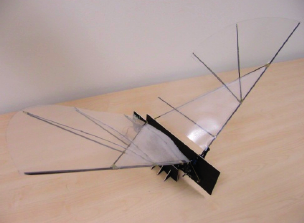
\includegraphics[scale=0.5]{p1.png}
\caption{ Flapping wing ornithopter prototype}
\label{fig:p1}
\end{figure}

It is important to make the mechanism as light as possible, therefore the lightest, and most cost
effective materials available are considered. Initially, carbon fiber which is strong and light-weight is one of the considerations. Due to limited resources to manufacture and cut carbon fibre and composites into the desired  shape, 3-D printing can be used for rapid prototying of the design. 3-D printing can be done with different  light-weight materials equivalent to carbon fibre/composite but not as durable.

There are several possible tools for cutting the carbon fiber (for instance: water jet and laser jet cutters), but the majority of manufacturers cut with rotary tools or straight blades. In rotary tools, an alternative to diamond cutter is the use of a "tungsten carbide" cutter, which allows to cut composite parts quicker, and  with less heat generation. After a piece has been cut, it is recommended to use Perma-Grit sanding blocks or hand tools to clean up the piece edges. 


\section{Conclusion}
Designing and developing a UAV is a multistage task which requires many iterations and stages. A typical wing designing process consists of airfoil selection, geometrical calculations, structural design, materials selection, numerical analysis and elaboration of technology. Composite materials prove to be very promising beacuse of their superior properties and light weight, amongst them polymer matrix composites are widely used inaviation industry characterize by high strength-to-weight and stiffness-to-weight ratio \citep{Grodzki}. But as the applications of drones are spreading different domains there is a need to look for more and more materials with extreme properties, for examples scientists have been using drones for studying and examining volcanic activities, here it becomes important to choose the materials wisely which have high temperature resistance, as in the future the drones may be occupying higher and higher altitudes leading to very low ro sub-zero amospheric temperatures .


\begin{figure}[h!]
\centering
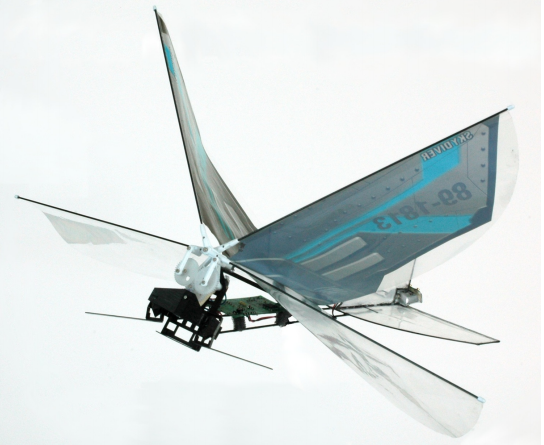
\includegraphics[scale=0.3]{dfm1}
\caption{Ornithopter (courtesy-Peterson et al)}
\end{figure}



\bibliographystyle{plain}
\bibliography{references}
\end{document}
